\chapter{Methoden}
\label{methods}
In diesem Kapitel wird aufgezeigt, wie die im Kapitel Einführung genannten Fragestellungen untersucht wurden.\\\\
Der Kern dieser Arbeit dreht sich um die folgende Frage: Verbessert sich ein CNN für eine spezifische Domäne, durch das hinzufügen domänenfremder Daten?
Konkret geht es darum, ob man annotierte domänenfremde Daten hinzuziehen kann, um ein CNN zu verbessern. Diese Fragestellung ist deshalb von Bedeutung, da es tendenziell immer zu wenig annotierte Daten gibt.
\section{Systemparameter}
\subsection{Hyperparameter}
\fixme{Hyperparametern}
\subsection{classweights}
\fixme{classweights}
\subsection{EarlyStopping}
\fixme{EarlyStopping}
\subsection{$F1_{pn}$ Score}
Um die Ergebnisse der Experimente zu vergleichen, wurde der positive und negative gemittelte $F1_{pn}$ Score gewählt. 
Der $F1_{pn}$ Score wird folgendermassen berechnet:\\
\begin{equation}
F1_{p|n} = 2*\frac{precission*recall}{precission+recalll}
\end{equation}\\
Der F1 Score wird für die positiven, wie auch die negativen Fälle berechnet und dann wie folgt gemittelt:\\
\begin{equation}
F1_{pn} = \frac{F1_p+F1_n}{2}
\end{equation}\\
Dieser Wert gilt als Standart um die Qualität einer binärer Klassifizierung zu messen. Der grosse Vorteil dieses Masses ist, dass durch eine einseitige, falsche Klassifizierung, der Wert sehr schlecht wird.
%TODO: Beispiel
\section{Word-Embeddings und Distant-Phase}
\subsection{Word-Embeddings}
Alle Experimente wurden mit 2 verschiedenen Word-Embeddings durchgeführt. Dabei soll der Einfluss, vielleicht auch eine Korrelation, zwischen den gewählten Word-Embedings und der Zieldomäne untersucht werden. Die Experimente wurden mit SemEval\_tweets und MPQ\_news Embeddings durchgeführt. Dass Tweets häufig aus vielen kurzen, teilweise auch stark abgekürzte Sätzen bestehen und News aus längeren, grammatikalisch korrekten Sätzen, wurde absichtlich so gewählt, damit allfällige Unterschiede im Resultat deutlicher sichtbar werden.
\subsection{Distant-Phase}
Aus der Arbeit \cite{deriu2016sentiment} ist ersichtlich, dass dieser Vorgang mit Tweets eine Verbesserung von fast 5 Prozentpunkte auf den $F1_{pn}$ Score erbrachte.
Deshalb wurde in dieser Arbeit eine Distant-Phase auf Reviews getestet. Alle nachfolgend beschrieben Experimente wurden einmal mit und einmal ohne einer Distanz-Phase auf Amazon Reviews durchgeführt.

\section{Aufbau der Experimente}
\label{experiments}
Die folgenden Experimente wurden jeweils für die Zieldomäne SemEval Tweets und MPQ Reviews durchgeführt. Bei allen Experimenten wird das CNN mit den gleichen Parametern initialisiert. Zusätzlich wurden alle Experimente drei Mal ausgeführt, um eine allfällige Varianz auszuschliessen.
\subsection{Experiment CrossDomain}
Mit dem Experiment V6 wurde die Kernfrage untersucht, ob die Performanz eines CNN steigt, wenn Domänenfremde Daten in die Trainingsphase mit einbezogen werden.
In einem ersten Schritt wurde das CNN mit domänenfremden Daten trainiert. Anschliessend wird das CNN in 20 Einzelschritten mit jeweils zusätzlich 400 Daten von der Zieldomäne weiter trainiert. Die genaue Aufteilung auf die verschiedenen Domänen ist im Bild \ref{fig:Method_V6} ersichtlich.
\begin{figure}[htbp][H]
	\centering
	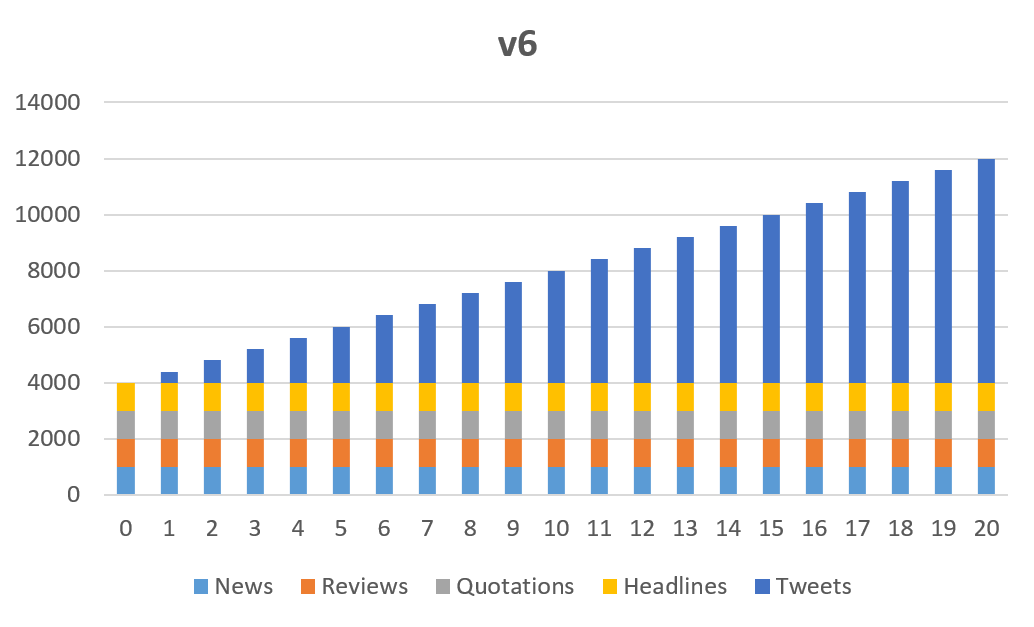
\includegraphics[width=0.7\textwidth]{img/Method_V6}
	\caption{Aufbau Experiment V6 - Tweets}
	\label{fig:Method_V6}
\end{figure}
Bei \ref{fig:Method_V6} ist die Zieldomäne SemEval Tweets, die Vorgehensweise für die Zieldomäne MPQ Reviews ist die Gleiche.
%TODO Bild wird am falschen Ort angezeigt
\subsection{Experiment SimilarDomain}
Im Experiment SimilarDomain wurde untersucht, wie stark sich die Performanz eines bereits trainierten CNN verbessert, wenn mit der Zieldomäne ähnlichen Daten weiter trainiert wird. Zum Beispielfür die Zieldomäne MPQ bedeuted dies, es wird ein CNN für die Zieldomäne MPQ Reviews trainiert. Anschliessend wird in 10 Teilschritten mit einer steigenden Anzahl anderer Review Domänen (siehe Kapitel Daten), weiter trainiert.
%TODO insert Picture

\subsection{Experiment BaseDomain}
\label{methods:v8}
Das Experiment BaseDomain dient als Baseline und somit Referenzwert für die Experimente CrossDomain und SimilarDomain.
Bei diesem Experiment wird nur mit den Daten der Zieldomäne trainiert und validiert \ref{fig:Method_V8}. Es dient als Anhaltspunkt, ob die Idee CrossDomain eine effektive  Steigerung der Performanz erbringen kann.
\begin{figure}[H]
	\centering
	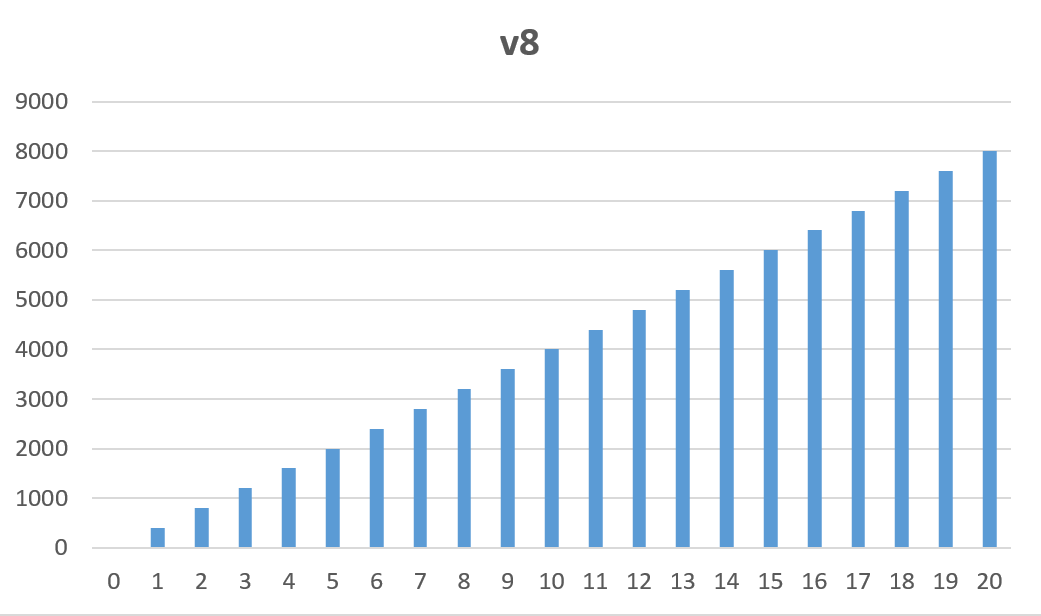
\includegraphics[width=0.7\textwidth]{img/Method_V8}
	\caption{Aufbau Experiment V8}
	\label{fig:Method_V8}
\end{figure}
\subsection{Namensgebung der Experimente}
Die 3 Experimente CrossDomain, SimilarDomain und BaseDomain wurden mit den zwei Zieldomänen MPQ\_news und SemEval\_tweets jeweils durchgeführt, zusätzlich wurden alle Experimente mit beiden Embeddings getestet und schlussendlich wurden alle Experimente einmal mit einer Distant-Phase und einmal ohne eine Distant-Phase ausgeführt. Da dies eine grosse Menge an Resultate liefert, ist nachfolgend die Namensgebung geregelt:

\begin{enumerate}  
	\item Wort - Experimenttyp (CrossDomain $\vert$ SimilarDomain $\vert$ BaseDomain)
	\item Wort - Zieldomäne (MPQ\_news $\vert$ SemEval\_tweets)
	\item Wort - Embeddings (newsEmb $\vert$ tweetEemb)
	\item Wort - Distant-Phase (withDP $\vert$ withoutDP)
	\item Wort - Ein einzelnes Experiment, oder eine ganze Experimentenreihe (0..200 $\vert$ all)
\end{enumerate}
Getrennt werden die einzelnen Wörter Angaben mit einem Bindestrich. Nachfolgend zwei Beispiele:
\begin{itemize}  
	\item CrossDomain-MPQ\_news-newsEmb-withDP-all
	\item SimilarDomain-SemEval\_tweets-tweetsEmb-withoutDP-200
\end{itemize}
Beim ersten Beispiel sind alle Experimente der Reihe CrossDomain, mit der Zieldomäne MPQ\_news, mit news Embeddings und einer Distant-Phase, von 0-200 Prozent gemeint. Das zweite Beispiel ist analog dem Ersten zu interpretieren, mit der Besonderheit, dass nur ein Experiment (dasjenige mit 200$\%$ Zieldomäne Daten) gemeint ist.

